\documentclass[a4paper, 14pt]{extarticle}
\usepackage[T1,T2A]{fontenc}
\usepackage[utf8]{inputenc}
\usepackage[english,ukrainian]{babel}
\usepackage{amsmath, amssymb, amsthm, mathtools}
\usepackage{bbm}
\usepackage{tikz}
\usetikzlibrary{positioning}
\usepackage{cancel}
\usepackage{graphicx}
\usepackage{color} 
\usepackage{hyperref}
\usepackage{xcolor}
\usepackage{pythonhighlight}
\hypersetup{
    colorlinks=true, %set true if you want colored links
    linktoc=all,     %set to all if you want both sections and subsections linked
    linkcolor=blue,  %choose some color if you want links to stand out
}
\usepackage{geometry}
 \geometry{
 a4paper,
 total={170mm,257mm},
 left=10mm,
 top=10mm,
 right=10mm
 }
\begin{document}

\begin{center}
    \topskip0pt
    \vspace*{\fill}
    \textsc{Київський національний університет імені Тараса Шевченка}\\
    \textsc{Факультет комп'ютерних наук та кібернетики}\\
    \vspace*{\fill}
    \textsc{Лабораторна робота №1}\\
    \textsc{з курсу "Проблеми багатозначного аналізу"}\\
    \vspace*{\fill}
    \begin{flushright}
        Виконала студентка групи ОМ-2\\
        Живолович Олександра Євгенівна\\
    \end{flushright}
    \vspace*{\fill}
    Київ, 2021
\end{center}
\thispagestyle{empty}

\newpage
\thispagestyle{empty}
\tableofcontents
\newpage

\section{Постановка задачі}
Побудувати графік субдиференціалу функції 
\begin{equation}
f(x_1,x_2) = |-4x_1+2x_2+4| + |2x_1+3x_2-2| + 0.1(x_1-3x_2)^6, \quad (x_1,x_2) \in \mathbb{R}^2.
\end{equation}
Розв'язати задачу 
\begin{equation}
    f(x_1,x_2) \to\min
\end{equation}
\begin{figure}[h]
    \centering
    \caption{Графік $f$}
    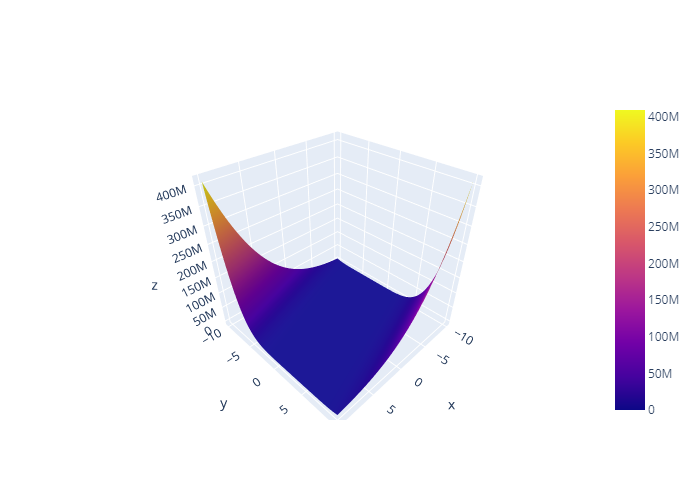
\includegraphics[width = \textwidth]{objective.png}
\end{figure}
\section{Субдиференціал}
\subsection{Теорія}
Для того, щоб знайти субдиференціал функції $f$,
скористаємося теоремою \\
Моро-Рокафеллера,
тобто 
\begin{equation*}
    \partial f(x) = \sum_{i=1}^3 \partial f_i(x)
\end{equation*}
де 
\begin{align*}
    f_1(x_1,x_2) &= |-4x_1+2x_2+4|\\
    f_2(x_1,x_2) &= |2x_1+3x_2-2|\\
    f_3(x_1,x_2) &= 0.1(x_1-3x_2)^6
\end{align*}
Розглянемо $f_1(x_1,x_2)$. Для того, щоб знайти субдиференціал 
у точці, де функція не є диференційовною
скористаємося теоремою Дубовітського - Мілютіна, тобто 
\begin{align*}
    \partial f_1(x_1,x_2)  
    &= \partial \max\{-4x_1+2x_2+4, 4x_1-2x_2-4\} = \partial
    \max\{f_{11}(x_1,x_2), f_{12}(x_1,x_2)\}=\\
    &= co\left(\bigcup_{i=1}^n \partial f_{1i}(x_1,x_2)\right)
\end{align*}
Тоді 
\begin{equation*}
    \partial f_1(x_1,x_2) = 
    \begin{cases}
        \{(-4,2)\}, 2x_2+4>4x_1\, \\
        \{(4,-2)\}, 2x_2+4<4x_1\, \\
        [(-4,2),(4,-2)],\, 2x_2 +4 =4x_1
    \end{cases}
\end{equation*}
Аналогічно для $f_2(x_1,x_2)$: 
\begin{equation*}
    \partial f_2(x_1,x_2) = 
    \begin{cases}
        \{(2,3)\}, 2x_1+3x_2-2>2\, \\
        \{(-2,-3)\}, 2x_1+3x_2-2<2\, \\
        [(-2,3),(2,-3)],\, 2x_1 +3x_2 -2 =2
    \end{cases}
\end{equation*}
Оскільки $f_3(x_1,x_2)$ диференційовна $\forall x\in\mathbb{R}^2$,
то її субдиференціал співпадає з градієнтом в усіх точках 
\begin{equation*}
    \partial f_3(x_1,x_2) = \{(0.6(x_1-3x_2)^5, -1.8(x_1-3x_2)^5)\}
\end{equation*}
\begin{figure}[h]
    \centering
    \caption{Субдиференціал}
    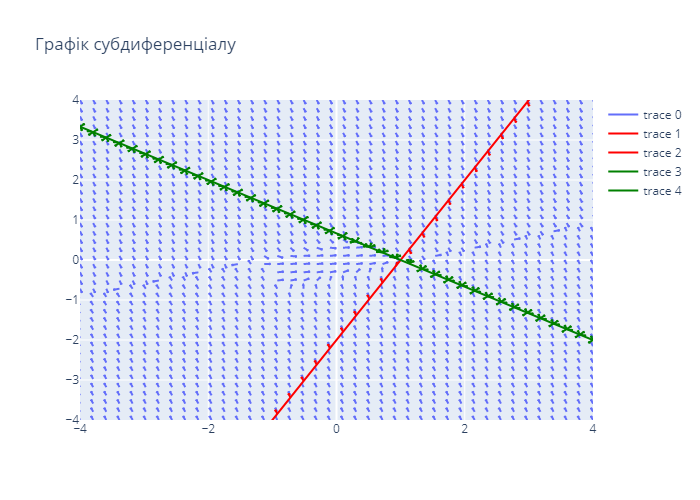
\includegraphics[width = \textwidth]{subdifferential.png}
\end{figure}
\newpage
\section{Алгоритм}
Нехай $f:\mathbb{R}^n\to\mathbb{R}$ опукла. Для мініміщації $f$,
використовуємо субградієнтний метод
\begin{equation}
    x_{k+1} = x_k - \alpha_k g(x_k)
\end{equation} 
де $x_k$ є $k$-тою точкою ітерації, $g(x_k)$ - будь-який субградієнт 
функції $f$ у точці $x_k$, $\alpha_k$ - розмір $k$-того кроку.

Отже, на кожному році методу, ми робимо крок у напрямку 
від'ємного субградієнту функції $f$. У точках, де 
$f$ диференційовна, субградієнт співпадає з градієнтом функції, а отже 
у цих точках метод зводиться до градієнтного методу.

Оскільки метод не є методом спуску, то гарним підходом 
є збереження найкращого поточного результату 
\begin{equation*}
    f^{(k)}_{\text{best}} = \min\{f^{(k-1)}_{\text{best}}, f^{(k)}\}
    \implies f^{(k)}_{\text{best}} =
    \min\{f(x_1),\hdots , f(x_k)\}.
\end{equation*}

Важливою частною методу є спосіб вибору $\alpha_k$ - розміру кроку.
Існують наступні широковживанні методи вибору $\alpha_k$:
\begin{itemize}
    \item Метод постійного розміру кроку
    \[
    \alpha_k = h    
    \]
    \item Метод кроку постійної довжини
    \[
    \alpha_k = \frac{h}{||g(x_k)||}    
    \]
    \item Метод сумовних з квадратом кроків
    \[
    \sum_{k=1}^\infty \alpha_k^2 <\infty, \quad 
    \sum_{k=1}^\infty \alpha_k = \infty
    \]
    Наприклад, $\alpha_k = a/(b+k), \, a>0,\,b\geq0$.
    \item Метод несумовних кроків, що зменшуються
    \[
        \lim_{k\to\infty}\alpha_k = 0,
        \quad\sum_{k=1}^\infty \alpha_k = \infty  
    \]
    Наприклад, $\alpha_k = a/\sqrt{k}$.
\end{itemize}
\section{Код}
Було обрано мову програмування \emph{Python3}, оскільки 
вона є дуже зручною для роботи з науковими обчисленнями,
а також існують багато зручних пакетів для візуалізації даних.
Код можна знайти за \href{https://github.com/Oleksandra-Zhyvolovych/multivariate-knu/tree/main/subgradient}{посиланням}.

Функціїї \pyth{plotObjective()} та \pyth{plotSubDiff()} будують 
графіки функції та субдиференціалу відповідно, за допомогою
програмного пакету \pyth{plotly}.

Усі обчисленнями виконується у функції \pyth{optimize}, що 
вирішує задачу негладкої оптимізації за допомогою 
субградієнтного методу. Функція має багато параметрів,
тобто є гнучкою у своії роботі, з багатьма значеннями,
виставленими за замовчуванням. 

Графіки для візуалізації результатів роботи алгоритму будуються за
домопомогою пакету \pyth{matplotlib}.

\newpage
\begin{python}
    def optimize(f,g,initial_point, strategy=Strategy.consant_size, h=0.1, a=1.0, 
    b=1.0, max_iterations=10000, tolerance=1e-6,
):
    points = []
    vals = []
    best_point = initial_point
    best_value = f(best_point)
    points.append(best_point)
    vals.append(best_value)

    step_size = 0.0
    for iter in range(1, max_iterations):
        if strategy == Strategy.consant_size:
            step_size = h
        elif strategy == Strategy.constant_length:
            step_size = h / np.linalg.norm(g(points[-1]))
        elif strategy == Strategy.square_summable:
            step_size = a / (iter + b)
        elif strategy == Strategy.diminishing:
            step_size = a / np.sqrt(iter)

        new_point = points[-1] - step_size * g(points[-1])
        new_value = f(new_point)
        points.append(new_point)
        vals.append(new_value)

        if new_value < best_value:
            best_point = new_point
            best_value = new_value
        if (
            abs(vals[-1] - vals[-2]) < tolerance
            and np.linalg.norm(points[-1] - points[-2]) < tolerance
        ):
            break

    return points, vals, best_point, best_value
\end{python}
\newpage
\section{Обчислювальні експерименти}
Сторонні математичні системи, такі як \emph{WolframAlpha},
знаходять мінімум функції у точці $(1.25665, 0.0133085)$,
зі значенням $f(x^\ast) = 0.877695$.
Розглянемо застосування субградієнтного методу з різними 
способами вибору кроку 
\subsection{Постійний розмір}
\begin{enumerate}
    \item $h=0.01$:  $x_{best} = (1.2511, 0.0065)$, $f(x_{best})=0.8792$, $\varDelta = 0.001$
    \item $h=0.001$: $x_{best} = (1.2549 0.0100)$,  $f(x_{best})= 0.8779$, $\varDelta=0.0002$
    \item $h=0.0001$: $x_{best} = (0.5993 0.0999)$  $f(x_{best})=3.3038$, $\varDelta = 2.4261$
\end{enumerate}
\subsection{Постійна довжина}
\begin{enumerate}
    \item $h=0.01  $:  $x_{best}=(1.2536, 0.0076)$, $f(x_{best})=0.8784$, $\varDelta=0.0007$
    \item $h=0.001 $:  $x_{best}=(0.9211, 0.0533)$, $f(x_{best})=1.4438$, $\varDelta=0.5661$
    \item $h=0.0001$:  $x_{best}=(0.0985, 0.0164)$, $f(x_{best})=6.3923$, $\varDelta=5.5146$
\end{enumerate}
\subsection{Сумовні з квадратом}
\begin{enumerate}
    \item $a=0.1, b=1.0$:   $x_{best})=( 1.2098, -0.0072)$, $f(x_{best})=0.8930$, $\varDelta = 0.01535$
    \item $a=0.05, b=1.0$:  $x_{best})=( 1.0966, -0.0449)$, $f(x_{best})=0.9307$, $\varDelta = 0.05306$
    \item $a=0.05, b=10.0$: $x_{best})=( 1.0573, -0.0380)$, $f(x_{best})=0.9536$, $\varDelta = 0.07592$
\end{enumerate}
\subsection{Несумовні, що зменшуються}
\begin{enumerate}
    \item $a=0.1  $: $x_{best}=(1.2537,  0.00752)$, $f(x_{best})=  0.8784$, $\varDelta= 0.0007$
    \item $a=0.05 $: $x_{best}=(1.2544,  0.00895)$, $f(x_{best})=  0.8781$, $\varDelta= 0.0004$
    \item $a= 0.01$: $x_{best}=(1.1841, -0.01580)$, $f(x_{best})=  0.9016$, $\varDelta= 0.0239$
\end{enumerate}
Візуалізації цих експериментів наведено у додатках.
\section{Висновки}
Була вирішена задача негладкої оптимізації за допомогою субградієнтного
методу. Були зроблені такі спостереження:
\begin{enumerate}
    \item Оскільки функція дуже швидко зростає, то 
    потрібно відразу брати малі кроки для того щоб метод був збіжний
    \item Надто малий розмір року призводить до вкрай повільної збіжності
    \item Методи постійного розміру кроку та 
    постійної довжини кроку показують гарні результати, але потребують 
    гарного підбору параметру.
    \item Метод сумовних з квадратом кроків показав гарний результат,
    навіть для не дуже вдалих параметрів.
    \item Метод несумовних кроків, що зменшуються показав 
    дуже гарний результат, але треба розуміти що зменшувати розмір 
    параметру потрібно обережно, адже можно швидко 
    прийти до дуже повільної збіжності.
\end{enumerate}
\newpage
\begin{thebibliography}{1}
\bibitem{1}
\emph{Subgradient Methods},
Stephen Boyd, Lin Xiao, and Almir Mutapcic
Notes for EE392o, Stanford University, Autumn, 2003
\end{thebibliography}
\newpage
\section{Додатки}
\begin{figure}[h]
    \centering
    \caption{Постійний розмір кроку}
    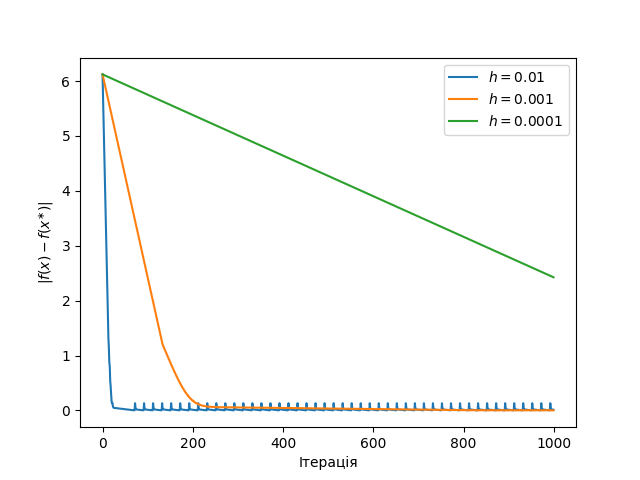
\includegraphics{const_size.png}
\end{figure}
\begin{figure}[h]
    \centering
    \caption{Постійна довжина кроку}
    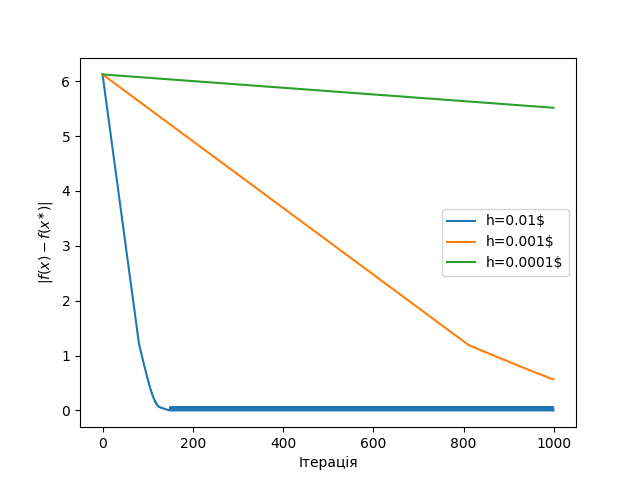
\includegraphics{const_len.png}
\end{figure}
\begin{figure}[h]
    \centering
    \caption{Сумовні з квадратом кроки}
    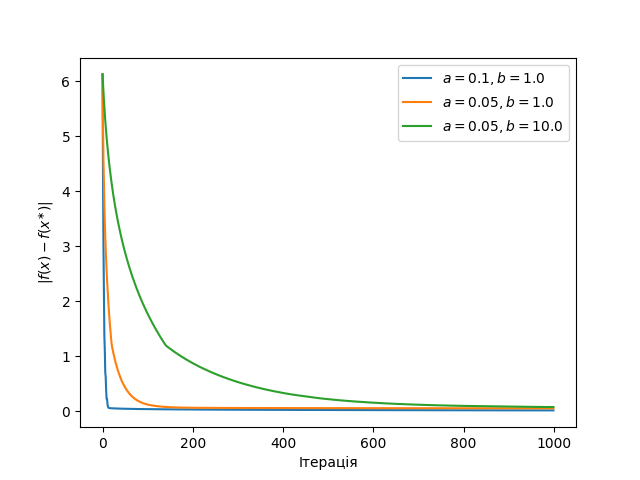
\includegraphics{square_summable.png}
\end{figure}
\begin{figure}[h]
    \centering
    \caption{Кроки, що зменшуються}
    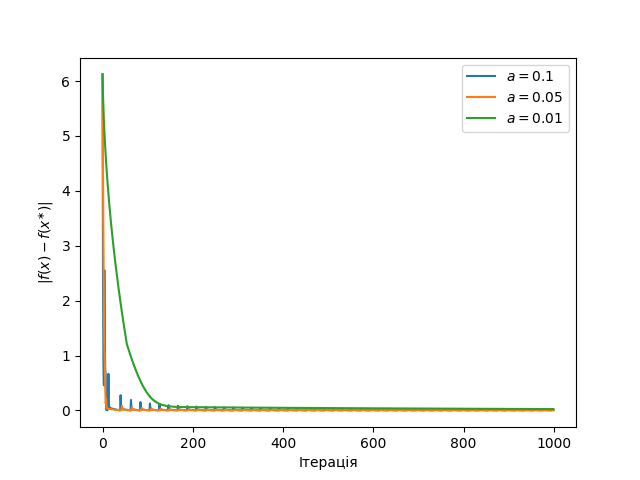
\includegraphics{diminishing.png}
\end{figure}
\end{document}